\documentclass{article}
\usepackage{cs170}
\begin{document}

\question{Study Group}
List the names and SIDs of the members in your study group.
If you have no collaborators, you must explicitly write “none”.

\question{Updating a MST}

You are given a graph $G = (V, E)$ with positive edge weights, and a minimum spanning tree $T = (V, E')$ with respect to these weights; you may assume $G$ and $T$ are given as adjacency lists. Now suppose the weight of a particular edge $e \in E$ is modified from $w(e)$ to a new value $\hat{w}(e)$. You wish to quickly update the minimum spanning tree $T$ to reflect this change, without recomputing the entire tree from scratch. 

There are four cases. In each, give a description of an algorithm for updating $T$, a proof of correctness, and a runtime analysis for the algorithm. Note that for some of the cases these may be quite brief. For simplicity, you may assume that no two edges have the same weight (this applies to both $w$ and $\hat{w}$).

\begin{subparts}
\subpart $e \notin E'$ and $\hat{w}(e) > w(e)$
\subpart $e \notin E'$ and $\hat{w}(e) < w(e)$
\subpart $e \in E'$ and $\hat{w}(e) < w(e)$
\subpart $e \in E'$ and $\hat{w}(e) > w(e)$
\end{subparts}

\question{Twenty Questions}
Your friend challenges you to a variant of the guessing game 20
questions. First, they pick some word $(w_1, w_2, ..., w_n)$ according
to a known probability distribution $(p_1, p_2, ..., p_n)$, i.e. word $w_i$
is chosen with probability $p_i$. Then, you ask yes/no questions until
you are certain which word has been chosen. You can ask any yes/no
question, meaning you can eliminate any subset $S$ of the possible
words with the question ``Is the word in $S$?''.

Define the cost of a guessing strategy as the expected number of
queries it requires to determine the chosen word, and let an optimal
strategy be one which minimizes cost. Design an $O(n \log n)$
algorithm to determine the cost of the optimal strategy.

\textbf{Give a 3-part solution.}

\emph{\textbf{Note:} We are only considering deterministic guessing
strategies in this question. Including randomized strategies doesn't
change the answer, but it makes the proof of correctness more
difficult.}

\question{Graph Game}

Given an undirected, unweighted graph $G$, with each node $v$ having a value $\ell(v) \geq 0$, consider the following game.
\begin{enumerate}
\item
All nodes are initially \emph{unmarked} and your score is $0$.
\item Choose an unmarked node $u$. Let $M(u)$ be the \emph{marked} neighbours of $u$.
Add $\sum_{v \in M(u)} \ell(v)$ to your score. Then mark $u$.
\item Repeat the last step for as many turns as you like, or until all the nodes are marked.
\end{enumerate}

For instance, suppose we had the graph:
\begin{figure}[h!]
\centering
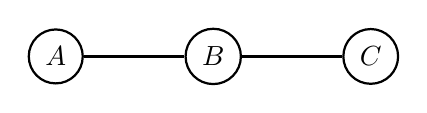
\begin{tikzpicture}[thick]
\node[draw,circle] (A) at (0,0) {$A$};
\node[draw,circle] (B) at (2,0) {$B$};
\node[draw,circle] (C) at (4,0) {$C$};

\draw (A) -- (B);
\draw (B) -- (C);
\end{tikzpicture}
\end{figure}

\noindent with $\ell(A) = 3$, $\ell(B) = 2$, $\ell(C) = 3$.
Then, an optimal strategy is to mark
$A$
then $C$
then $B$
giving you a score of
$0+0+6$.
We can check that no other order will give us a better score.

\begin{subparts}
\subpart Is the following statement true or false? \textbf{For any graph, an optimal strategy which marks all the vertices always exists.} Briefly justify your answer.
\subpart Give a greedy algorithm to find the order which gives the best score. \textbf{Please give a 3-part solution for this part.}
\subpart Now suppose that $\ell(v)$ can be negative. Give an example where your algorithm fails.
\subpart Your friend suggests the following modified algorithm: delete all $v$ with $\ell(v) < 0$,
then run your greedy algorithm on the resulting graph. Give an example where this algorithm fails.
\end{subparts}

\end{document}